\chapter{Approximations of VIX options}

% In this section, we use the methods illustrated before to price options under several volatility models. In section \ref{sec: 3.1}, we approximate option prices with 1-dimensional volatility processes; In section \ref{sec: 3.2}, method is given to price options under double CEV model. In section \ref{sec: 3.3}, while pricing path-dependent options like American options, we use the DOI estimator and shows that it's able reduce simulations' variance.

\section{Approximating options under mean-reverting CEV model}
\label{sec: 3.1}

\subsection{Drawbacks of using Black-Scholes model as an auxiliary model}
\cite{chan_empirical_1992} proposes the mean-reversion CEV model, in which volatility follows

$$
    d V_{t}=\left(\alpha+\beta V_{t}\right) d t+\sigma V_{t}^{\gamma} d W_{t}
$$

\noindent when $\beta$ is negative, this model has mean-reverting property. We can rewrite it to be

\begin{equation}\label{mr}
    d V_t=\kappa(m - V_t) d t+\sigma V^{\gamma}_t d W_t
\end{equation}

\noindent where $\kappa$ is the speed of mean-reversion, $m$ is the long-run mean. A natural idea is to use Black-Scholes model as auxiliary model as mentioned in \cite{kristensen_adding_2011}, then apply their method to approximate the VIX option price under mean-reverting CEV model. Denote $\mathcal{L}$ and $\mathcal{L}^{\text{BS}}$ to be infinitesimal generators of mean-reverting CEV model and Black-Scholes model respectively

$$
\begin{aligned}
    \mathcal{L} w&= \frac{\partial w}{\partial t}+\kappa(m - V) \frac{\partial w}{\partial V}+\frac{1}{2} \sigma^{2} V^{2\gamma} \frac{\partial^{2} w}{\partial V^{2}} \\
    \mathcal{L}^{\text{BS}} w &= \frac{\partial w}{\partial t}+rV \frac{\partial w}{\partial V}+\frac{1}{2} \sigma^{2} V^2 \frac{\partial^{2} w}{\partial V^{2}}
\end{aligned}
$$

\noindent The mis-pricing term for using Black-Scholes model is then

$$\delta^{\text{BS}} = (\mathcal{L} - \mathcal{L}^{\text{BS}}) w^{\text{BS}} = (\kappa - r)V \frac{\partial w^{\text{BS}}}{\partial t} + \kappa m \frac{\partial w^{\text{BS}}}{\partial t} + \sigma^{2} (V - V^{2 \gamma}) \frac{\partial^{2} w^{\text{BS}}}{\partial V^{2}} $$

\noindent with the solution of Black-Scholes model $w^{\text{BS}}$. Note that $\delta^{\text{BS}}$ contains theta and gamma of option. Their differences in Black-Scholes model and mean-reverting model determines that we have to use other auxiliary models.

Take call option prices under $\gamma=\frac{1}{2}$ in model\eqref{mr} as an example. This model is known as mean square root mean-reverting model proposed by \cite{grunbichler_valuing_1996}.


\begin{figure}[ht]
    \centering
    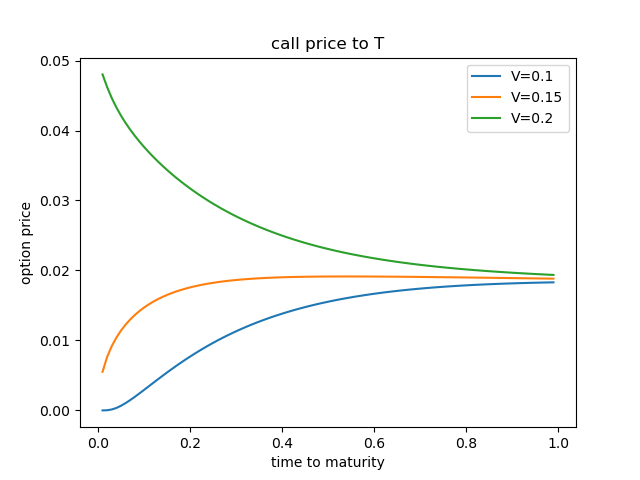
\includegraphics[width=10cm]{./figures/call2T.png}
    \caption{Call option price with regard to time to maturity}\label{call2t}
\end{figure}

\begin{figure}[ht]
    \centering
    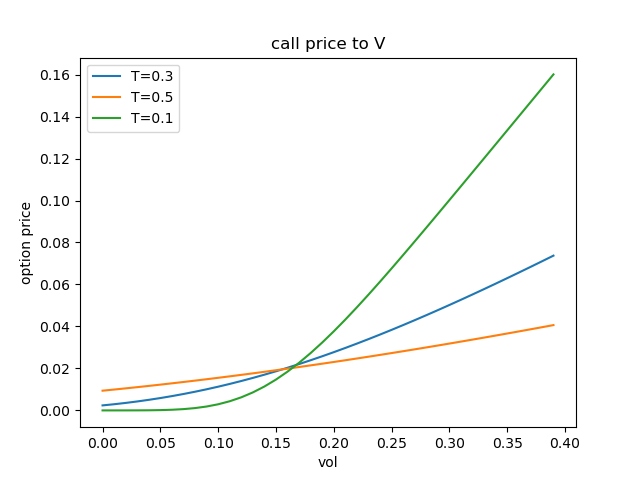
\includegraphics[width=10cm]{./figures/call2V.png}
    \caption{Call option price with regard to volatility}\label{call2v}
\end{figure}

From figure \ref{call2t}, we can find that in contrast to Black-Scholes model, the value of call option price under mean-reverting model is not always increasing as time to maturity increases; From figure \ref{call2v}, by contrast, the call option price does not converge to zero as volatility goes to zero. In addition, \cite{grunbichler_valuing_1996} also shows that $V$ has less influence of the current value of the call option than in Black-Scholes model. For these reasons, we conclude that Black-Scholes model is not an appropriate auxiliary model and in the next section, we discuss that using the square root mean-reverting model as the auxiliary model.

\subsection{Using square root mean-reverting model as auxiliary model}

Recall the mean-reverting CEV model with $\gamma=\frac{1}{2}$

\begin{equation}
    d V_t=\kappa(m - V_t) d t+\sigma \sqrt{V_t} d W_t
\end{equation}

We are going to use it as our auxiliary model as it captures the mean-reverting property of general mean-reverting CEV models. \cite{grunbichler_valuing_1996} gives an explicit solution to this model. Denote the call option price $\bar{w}$ with strike $K$, constant risk-free rate $r$, time to maturity $T$ and no expected premium for volatility risk is paid, its price is given by

\begin{equation}\label{aux call price}
    \begin{aligned}
        \bar{w}=&  e^{ -(\kappa+r) T} V Q(x K ; \nu+4, \lambda) \\
        &+ m e^{-r T}(1-e^{-\kappa T}) Q(xK ; \nu+2, \lambda) \\
        &-e^{-r T} K Q(x K; \nu, \lambda)
        \end{aligned}
\end{equation}

\noindent where

$$
\begin{aligned}\label{para}
    &x=\frac{4 \kappa}{\sigma^{2}(1-e^{-\kappa T})} \\
    &\nu=\frac{4 \kappa m}{\sigma^{2}}, \\
    &\lambda= e^{-\kappa T}x V
    \end{aligned}
$$

\noindent and $Q(xK ; \nu+i, \lambda)$ is the complementary distribution function for the non-central chi-squared density with $\nu + i$ degrees of freedom and non-centrality parameter $\lambda$.

Define the infinitesimal generators $\bar{\mathcal{L}}$ for square root mean-reverting model and $\mathcal{L}$ for mean-reverting CEV model

\begin{equation}\label{inf gen1}
    \begin{aligned}
        \mathcal{L} w&= \frac{\partial w}{\partial t}+\kappa(m - V) \frac{\partial w}{\partial V}+\frac{1}{2} \sigma^{2} V^{2\gamma} \frac{\partial^{2} w}{\partial V^{2}} \\
        \bar{\mathcal{L}} w &= \frac{\partial w}{\partial t}+\kappa(m - V) \frac{\partial w}{\partial V}+\frac{1}{2} \sigma^{2} V \frac{\partial^{2} w}{\partial V^{2}}
    \end{aligned}
\end{equation}

Subtract infinitesimal generators in equation\eqref{inf gen1}, we get the mis-pricing formula for using square root mean-reverting model

$$
\delta = (\mathcal{L} - \bar{\mathcal{L}}) \bar{w} = \frac{1}{2} \sigma^{2} (V^{2\gamma} - V) \frac{\partial^{2} w}{\partial V^{2}}
$$

\noindent We can then use the approximation formula discussed in \ref{sec: 2.2} to price call options under mean-reverting CEV model\footnote{Put options can be priced easily in the same way}

\begin{equation} \label{cev approx formula}
    w_{N}(t, x)=\bar{w}(t,x)+\sum_{n=0}^{N} \frac{(T-t)^{n+1}}{(n+1) !} \delta_{n}(t, x)
\end{equation}

\noindent where

\begin{equation}\label{mispricing}
    \begin{aligned}
        &\delta_0 = \delta = \frac{1}{2} \sigma^{2} (V^{2\gamma} - V) \frac{\partial^{2} w}{\partial V^{2}} \\
        &\delta_{n}(t, x)=L \delta_{n-1}(t, x)- r\delta_{n-1}(t, x)
        \end{aligned}
\end{equation}

Finally we get a closed form approximating formula for call options under mean-reverting CEV model. But notice that the call price \eqref{aux call price} contains non-square chi square distribution functions, applying infinitesimal generator $\mathcal{L}$ on it can be a hard point and in the next section we are going to talk about how to derive partial derivatives of distribution function $Q(xK; \nu+i, \lambda)$.

\subsection{Method to Calculate Derivatives In Expansions}

In this section, methods to calculate closed-form partial derivatives of call option price $\bar{w}$ to time $t$ and volatility $V$. Our method is based on the recurrence relation of non-central chi-square distribution proposed by \cite{cohen_noncentral_1988}, which is

\begin{equation}\label{pdf diff}
    \begin{gathered}
        \frac{\partial p(xK;\nu,\lambda)}{\partial (xK)}=\frac{1}{2}[-p(xK ; \nu, \lambda)+p(xK ; \nu-2, \lambda)]\\
        \frac{\partial p(xK;\nu,\lambda)}{\partial \lambda}=\frac{1}{2}[-p(xK ; \nu, \lambda)+p(xK ; \nu+2, \lambda)] \\
    \end{gathered}
\end{equation}

\noindent where $p(xK;\nu,\lambda)$ is the Probability Density Function(PDF) of non-central chi-square distribution. From the relationship between Complementary Cumulative Distribution Function(CCDF) $Q(xK;\nu,\lambda)$, Cumulative Distribution Function(CDF) $F(xK;\nu,\lambda)$, and PDF we know that

\begin{equation}\label{CCDF2x}
    \begin{aligned}
        \frac{\partial Q(xK; \nu, \lambda)}{\partial (xK)}&=\frac{\partial[1-F(xK; \nu, \lambda)]}{\partial (xK)} \\ 
        &=-\frac{\partial F(xK; \nu, \lambda)]}{\partial (xK)}\\
        &= -p(xK;\nu,\lambda)
    \end{aligned}
\end{equation}

\noindent Rewrite the second equation in \eqref{pdf diff}, we get

\begin{equation}\label{pdf trans}
    \begin{aligned}
        \frac{\partial p(xK;\nu,\lambda)}{\partial \lambda}&=\frac{1}{2}[-p(xK ; \nu, \lambda)+p(xK ; \nu+2, \lambda)] \\
        &=-\frac{1}{2}[-p(xK ; \nu+2, \lambda)+p(xK ; \nu, \lambda)]\\
        &= -\frac{\partial p(xK;\nu+2,\lambda)}{\partial (xK)}
    \end{aligned}
\end{equation}

\noindent Integrate both sides of \eqref{pdf trans} with respect to $xK$ and combine with \eqref{CCDF2x}, we can derive the partial derivative of CDF to non-central parameter $\lambda$

\begin{equation}
    \begin{aligned}
        \frac{\partial}{\partial \lambda} F(xK;\nu,\lambda)&=-\frac{\partial}{\partial (xK)}F(xK;\nu+2,\lambda) \\
        &= -p(xK;\nu+2,\lambda)
    \end{aligned}
\end{equation}

\noindent Finally we get the partial derivative of CCDF to non-central parameter $\lambda$

\begin{equation}\label{CCDF2lambda}
    \begin{aligned}
        \frac{\partial Q(xK; \nu, \lambda)}{\partial \lambda}&=\frac{\partial[1-F(xK; \nu, \lambda)]}{\partial \lambda} \\ 
        &=-\frac{\partial F(xK; \nu, \lambda)]}{\partial \lambda}\\
        &= p(xK;\nu+2,\lambda)
    \end{aligned}
\end{equation}

Until now we can summarize that the derivatives of CCDF and PDF are all combinations of PDFs with change of degrees of freedom. Without loss of accuracy, we make the degrees of freedom in PDF be consistent with call option solution in \eqref{aux call price}, that is for $p(xK;\nu+i, \lambda)$, we let $i \in [0,4]$. Use the non-central chi-square property by \cite{cohen_noncentral_1988} to do the following transformation

\begin{equation}\label{trans}
    \begin{aligned}
        p(xK ; \nu-2, \lambda)&=\frac{\lambda}{xK} p(xK ; \nu+2, \lambda)+\frac{v-2}{xK} p(xK ; \nu, \lambda) \\
        p(xK ; \nu+6, \lambda)&=\frac{xK}{\lambda} p(xK ; \nu+2, \lambda)-\frac{\nu+2}{\lambda} p(xK ; \nu+4, \lambda)
    \end{aligned}
\end{equation}

Next we use the results above to calculate delta and gamma of auxiliary call option price $\bar{w}$. Recall the parameter $xK$, $\nu$ and $\lambda$ in \eqref{para}, where

\begin{equation}
    \begin{aligned}
        &x=\frac{4 \kappa}{\sigma^{2}(1-e^{-\kappa T})} \\
        &\nu=\frac{4 \kappa m}{\sigma^{2}}, \\
        &\lambda= e^{-\kappa T}x V
    \end{aligned}
\end{equation}

\noindent Then we use chain rule calculate the following auxiliary derivatives

\begin{equation}
    \begin{aligned}
        \frac{\partial Q(xK; \nu, \lambda)}{\partial V}&= \frac{\partial Q}{\partial x}\frac{\partial x}{\partial V} + \frac{\partial Q}{\partial \lambda} \frac{\partial \lambda}{\partial V} \\
        &=0 + x e^{-\kappa T} p(x ; \nu+2, \lambda)\\
        &= x e^{-\kappa T} p(x ; \nu+2, \lambda)
    \end{aligned}
\end{equation}

\noindent Thus delta is given by

\begin{equation}
    \begin{aligned}
        \Delta_{\bar{w}}=&  e^{ -(\kappa+r) T} Q(x K ; \nu+4, \lambda) + e^{ -(\kappa+r) T}V \cdot x e^{-\kappa T} p(x K ; \nu+6, \lambda)\\
        &+ m e^{-r T}(1-e^{-\kappa T}) \cdot x e^{-\kappa T} p(x ; \nu+2, \lambda) -e^{-r T} K \cdot x e^{-\kappa T} p(x ; \nu+2, \lambda)
        \end{aligned}
\end{equation}

\noindent Using \eqref{trans} to substitute $p(xK;\nu+6,\lambda)$ and simplify the equation

\begin{equation}
    \begin{aligned}
        \Delta_{\bar{w}}=&  e^{ -(\kappa+r) T} Q(x K ; \nu+4, \lambda) \\
        &+ e^{ -(\kappa+r) T} \lambda \left[\frac{xK}{\lambda} p(xK ; \nu+2, \lambda)-\frac{\nu+2}{\lambda} p(xK ; \nu+4, \lambda)\right]\\
        &+ m e^{-r T}(1-e^{-\kappa T}) \cdot \frac{4 \kappa}{\sigma^{2}(1-e^{-\kappa T})} e^{-\kappa T} p(x ; \nu+2, \lambda) -e^{-(r+\kappa) T} K  p(x ; \nu+2, \lambda) \\
        =& e^{ -(\kappa+r) T} [Q(x K ; \nu+4, \lambda)-2p(x K ; \nu+4, \lambda)] 
        \end{aligned}
\end{equation}

% \begin{figure}[ht]
%     \centering
%     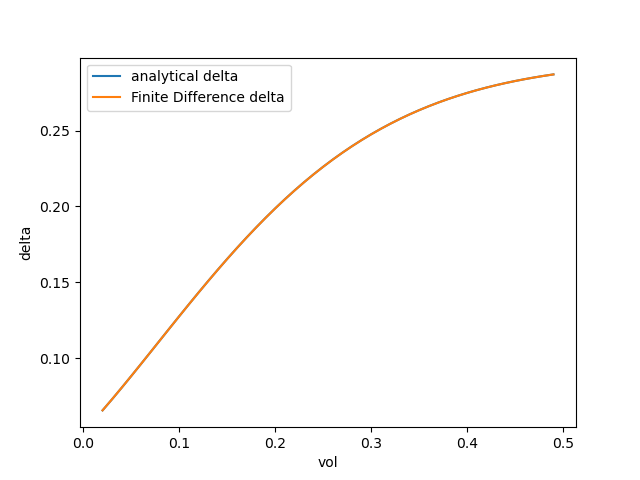
\includegraphics[width=10cm]{./figures/delta_comparison.png}
%     \caption{delta comparison, computed by our formula and discretisation}\label{delta comparison}
% \end{figure}

% \begin{figure}[ht]
%     \centering
%     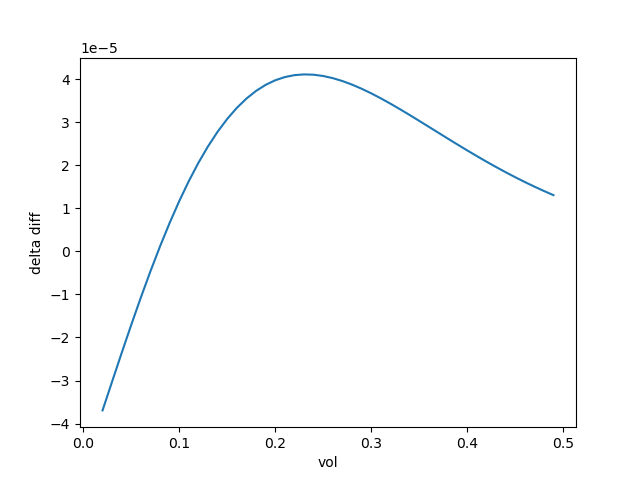
\includegraphics[width=10cm]{./figures/delta_diff.png}
%     \caption{delta differences}\label{delta diff}
% \end{figure}

\begin{figure}[!tbp]
    \centering
    \subfloat[delta comparison]{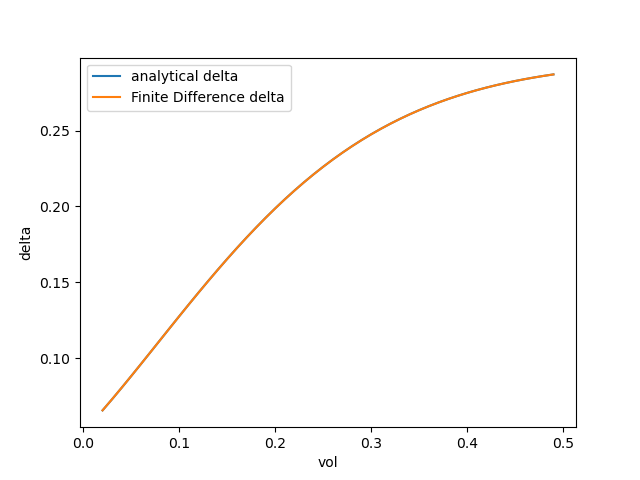
\includegraphics[width=0.8\textwidth]{./figures/delta_comparison.png}\label{delta comparison}}
    \hfill
    \subfloat[delta differences between two methods]{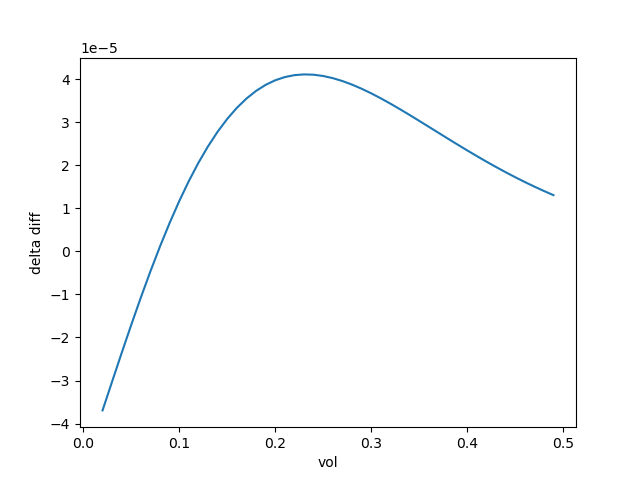
\includegraphics[width=0.8\textwidth]{./figures/delta_diff.png}\label{delta diff}}
    \caption{Deltas are calculated by our formula, and take call option price differences and divided by vol differences. The parameters used are $T=0.3$,$\alpha = 0.60$, $\beta = 4.00$, $\sigma = 0.133$, $r = 0.05$, and $K= 0.15$.  }
  \end{figure}


\noindent Similarly, we calculate another auxiliary derivative

\begin{equation}
    \begin{aligned}
        \frac{\partial p(xK;\nu,\lambda)}{\partial V} &= \frac{\partial p}{\partial (xK)}\frac{\partial (xK)}{\partial V} + \frac{\partial p}{\partial \lambda} \frac{\partial \lambda}{\partial V} \\
        &= \frac{x e^{-\kappa T}}{2} [-p(xK ; \nu, \lambda)+p(xK ; \nu+2, \lambda)]
    \end{aligned}
\end{equation}

\noindent As a result, gamma of $\bar{w}$ is then

\begin{equation}\label{gamma}
    \begin{aligned}
        \Gamma_{\bar{w}}&= e^{ -(\kappa+r) T} \left[x e^{-\kappa T} p(x ; \nu+6, \lambda)-2 \cdot \frac{x e^{-\kappa T}}{2} [-p(xK ; \nu, \lambda)+p(xK ; \nu+2, \lambda)]\right] \\
        &= xe^{ -(2\kappa+r) T}p(xK;nu+4,\lambda)
    \end{aligned}
\end{equation}

To apply infinitesimal generator on mis-pricing formula, we still need to calculate partial derivatives of PDF to time $t$. Define the following auxiliary functions

\begin{equation}
    \begin{aligned}
        \frac{\partial (x K)}{\partial t}&= \frac{-\kappa e^{-\kappa T}}{1 - e^{-\kappa T}} \cdot  xK\\
        \frac{\partial \lambda}{\partial t}& =\frac{-\kappa e^{-\kappa T}}{1 - e^{-\kappa T}} \cdot  xV
    \end{aligned}
\end{equation}

\noindent Then partial derivatives of PDF to $t$ is given by

\begin{equation}
    \begin{aligned}
        \frac{\partial p(xK; \nu, \lambda)}{\partial t}&= \frac{\partial p}{\partial (xK)}\frac{\partial (xK)}{\partial t} + \frac{\partial p}{\partial \lambda} \frac{\partial \lambda}{\partial t} \\
        &= \frac{-\kappa x e^{-\kappa T}}{2(1 - e^{-\kappa T})} \left[Vp(xK ; \nu+2, \lambda) - (K+V) p(xK ; \nu, \lambda) + K p(xK ; \nu-2, \lambda)\right]\\
    \end{aligned}
\end{equation}

From \eqref{mispricing} we know that the mis-pricing formula $\delta = \frac{1}{2} \sigma^2 (V^{2\gamma}-V) \Gamma_{\bar{w}}$, all terms in which have been solved from above. In essence, to apply Ito-Taylor expansions on $\delta$, we use the following algorithm as used in calculating delta and gamma:

\begin{enumerate}
    \item Combining previous auxiliary partial derivatives, use chain rule to apply infinitesimal generator on mis-pricing formula.
    \item Substitute PDFs with noncentral parameter $\nu+i$ where $\nu \notin [0,4]$.
    \item Back to step 1, apply higher order infinitesimal generators.
\end{enumerate}

Therefore, we illustrate a solution to implement approximation method on volatility options under mean-reverting CEV model. The expansions in approximating formula can be computed once for all, we can solve it manually or use symbolic language for higher orders. All terms in the result is explicit expect non-central chi-square PDFs, we plug $p(xK;\nu+i,\lambda)$ into the result at last.

\section{Approximating options under double Heston model}

\cite{gatheral_consistent_nodate} proposes volatility with double mean-reverting dynamics

$$
    \begin{aligned}
        d V_t &=-\kappa\left(V_t-V^{\prime}(t)\right) d t+\eta_{1} V^{\prime \alpha}_t  d W_1(t) \\
        d V^{\prime}_t &=-c\left(V^{\prime}_t-m\right) d t+\eta_{2} V^{\prime \beta}_t d W_{2}(t)
    \end{aligned}
$$

\noindent where $\alpha, \beta \in [\frac{1}{2},1]$.

\begin{itemize}
    \item It's called Double Heston model in the case $\alpha=\beta=\frac{1}{2}$.
    \item The case $\alpha=\beta=1$ Double Log-normal model.
    \item And the general Double CEV model.
\end{itemize}

From our previous work, we can use the same auxiliary model to price options with $V_t$ following heston dynamics and $V^{\prime}_t$ following any mean-reverting CEV process, we call it one Heston one CEV model. This model is given by

\begin{equation}\label{heston cev}
    \begin{aligned}
        d V_t &=-\kappa\left(V_t-V^{\prime}(t)\right) d t+\eta_{1} \sqrt{V_t} d W_1(t) \\
        d V^{\prime}_t &=-c\left(V^{\prime}_t-m\right) d t+\eta_{2} V^{\prime \beta}_t d W_{2}(t)
    \end{aligned}
\end{equation}

Define infinitesimal generator $\mathcal{L}$ for \eqref{heston cev} and $\bar{\mathcal{L}}$ for square root mean-reverting model

\begin{equation}\label{inf gen2}
    \begin{aligned}
        \mathcal{L} w&= \frac{\partial w}{\partial t}+\kappa(V^{\prime} - V) \frac{\partial w}{\partial V}+\frac{1}{2} \eta_1^{2} V \frac{\partial^{2} w}{\partial V^{2}} \\
        &+ \frac{\partial w}{\partial t}+c(m^{\prime} - V^{\prime}) \frac{\partial w}{V^{\prime}}+\frac{1}{2} \eta_2^{2} V \frac{\partial^{2} w}{V^{\prime 2}}\\
        \bar{\mathcal{L}} w &= \frac{\partial w}{\partial t}+\kappa(m - V) \frac{\partial w}{\partial V}+\frac{1}{2} \eta_1 V \frac{\partial^{2} w}{\partial V^{2}}
    \end{aligned}
\end{equation}

\noindent Mis-pricing formula for it is then

$$
\begin{aligned}
    \delta = (\mathcal{L} - \bar{\mathcal{L}}) \bar{w} &= \kappa(V^{\prime}-m)\frac{\partial w}{\partial V} \\
    &= \kappa(V^{\prime}-m) \Gamma_{\bar{w}}
\end{aligned}
$$

\noindent where $\Gamma_{\bar{w}}$ is given in \eqref{gamma}.